%!TEX root = tesis.tex
\chapter{Aprendizaje en un \ssolver paralelo y distribuido}
\label{aprendizaje-pardist}


\section{¿Cómo compartir cláusulas aprendidas?}

Hemos observado que la partición de un problema en subproblemas a menudo conlleva una dosis considerable de retrabajo, y hemos conjeturado que el aprovechamiento de las cláusulas aprendidas durante el análisis parcial de un problema difícil es importante para eliminar (o al menos mitigar el impacto negativo de) dicho retrabajo. Para llevar a la práctica una serie de experimentos que permitan poner a prueba esta hipótesis es necesario tomar ciertas decisiones importantes acerca de:

\begin{itemize}
\item cómo deberían compartirse las cláusulas aprendidas
\item con quién(es) y/o entre quién(es)
\item cuándo y/o cada cuánto
\item cuántas y/o cuáles
\end{itemize}

\subsubsection{Consideraciones de escalabilidad}

Queremos evitar cualquier enfoque que introduzca nuevos cuellos de botella en la arquitectura. Por ejemplo, no sería aceptable la incorporación de una gran base de datos centralizada en la que todos los \ws almacenen las cláusulas que van aprendiendo y que todos los \ws deban consultar.

Tampoco sería aceptable un grafo completo de comunicación permanente para lograr ese mismo fin, es decir, hacer que cada \w le comunique (o consulte) a todos los demás las cláusulas que va(n) aprendiendo.


\subsubsection{Independencia del \ssolver particular utilizado}

Como ya hemos recalcado en el Cap.~\ref{}, nos interesa que el \ssolver que utiliza cada uno de los \ws sea fácil de actualizar y/o de reemplazar por otro componente \ots similar. Si bien suelen ser necesarios algunos cambios para lograr que un \ssolver permita la inyección \emph{inicial} de cláusulas aprendidas (en lugar de comenzar sin ninguna), por lo general tales cambios se reducen a cuestiones de interfaz y no revisten mayor dificultad.

Es más ambicioso, en cambio, pretender poder inyectar nuevas cláusulas aprendidas en cualquier momento \emph{durante} el proceso de búsqueda. Para ello habría que introducir modificaciones mucho más fuertemente acopladas a la versión particular de \ssolver en uso, sus algoritmos, estructuras de datos e invariantes particulares.


\subsubsection{Influencia del esquema de particionamiento}

El enfoque de particionamiento recursivo, basado en \emph{guiding paths}, que hemos adoptado para la construcción de la herramienta también influye en la elección de un mecanismo adecuado para compartir información de cláusulas aprendidas. Recordemos que cada subproblema es identificable con un camino único de literales (las variables levantadas, con cierta combinación particular de valores de verdad asignados). De hecho, si esperamos que los análisis de subproblemas sean cada vez más fáciles en comparación con los de sus padres es justamente debido a que una mayor cantidad de variables proposicionales han dejado de ser variables para convertirse en constantes.

Debido a lo antedicho, no es evidente que una cláusula aprendida durante el análisis de cierto subproblema deba necesariamente ser una cláusula aprendida válida a la hora del análisis de otros subproblemas arbitrarios (que no sean parte de su descendencia, es decir, que no tengan el camino de literales del subproblema donde se aprendió originalmente la cláusula como prefijo del suyo propio).


\subsubsection{Entonces \ldots}

Como consecuencia de los factores anteriormente expuestos, vemos que resulta natural considerar la \emph{herencia} de cláusulas aprendidas del problema padre a sus subproblemas hijos como metodología para compartir conocimiento de manera controlada \ldots ojalá acumulable \ldots etc \ldots


\subsubsection{¿Y cuántas/cuáles heredamos\ldots?}

Que cada hijo herede TODAS las cláusulas aprendidas por su padre probablemente sea demasiado / contraproducente:
\begin{itemize}
\item Por algo los solvers secuenciales van purgando: es sabido que zarparse no es bueno.
\item OK, el padre sí llegó a todo eso, pero por algo los solvers secuenciales van subiendo de a poco el máximo de aprendidas: es sabido que zarparse desde el primer momento no es buena idea. Y estamos suponiendo que los subproblemas serán más chicos/fáciles que su problema padre.
\item Y además, la herencia no es inmediata sino mediata. Jugarse a heredar todo implica jugarse a pagar el precio de bajar todo eso a disco, guardar todo eso en storage/pending, leer todo eso de disco, etc. Bocha overhead.
\end{itemize}

Por lo tanto vamos a necesitar criterios de selección, subconjunto, etc.


\section{Prueba de concepto}

\subsubsection{Objetivos y metodología}

Acá explicamos para qué y de qué modo se llevaron a cabo estos experimentos preliminares. Que son una aproximación de orden cero a lo que podría obtenerse en un cluster posta haciendo todo recursivamente, que permiten evaluar a grosso modo la factibilidad de la idea, etc, etc.

\subsubsection{Resultados obtenidos}

Acá van los resultados de las perchitas.

\subsubsection{Discusión y conclusiones}

Acá discutimos los resultados y concluimos que vale la pena probar implementar la herencia de cláusulas aprendidas en modo paralelo y distribuido, y evaluarla en un cluster posta.


\section{Resultados experimentales}

En esta sección vamos a presentar los resultados posta de los experimentos ejecutados en distribuido.

\subsection{Criterios de selección de cláusulas}

Descripción de los distintos criterios \ldots

\subsection{Resultados obtenidos}

\subsubsection{Garping del mejor criterio para cada problema}

\subsubsection{Promedios por cada criterio}

\subsubsection{Heatmaps para scopes crecientes}


\subsection{Discusión y conclusiones}


\newpage
% \begin{figure}
% 	\centering
% 	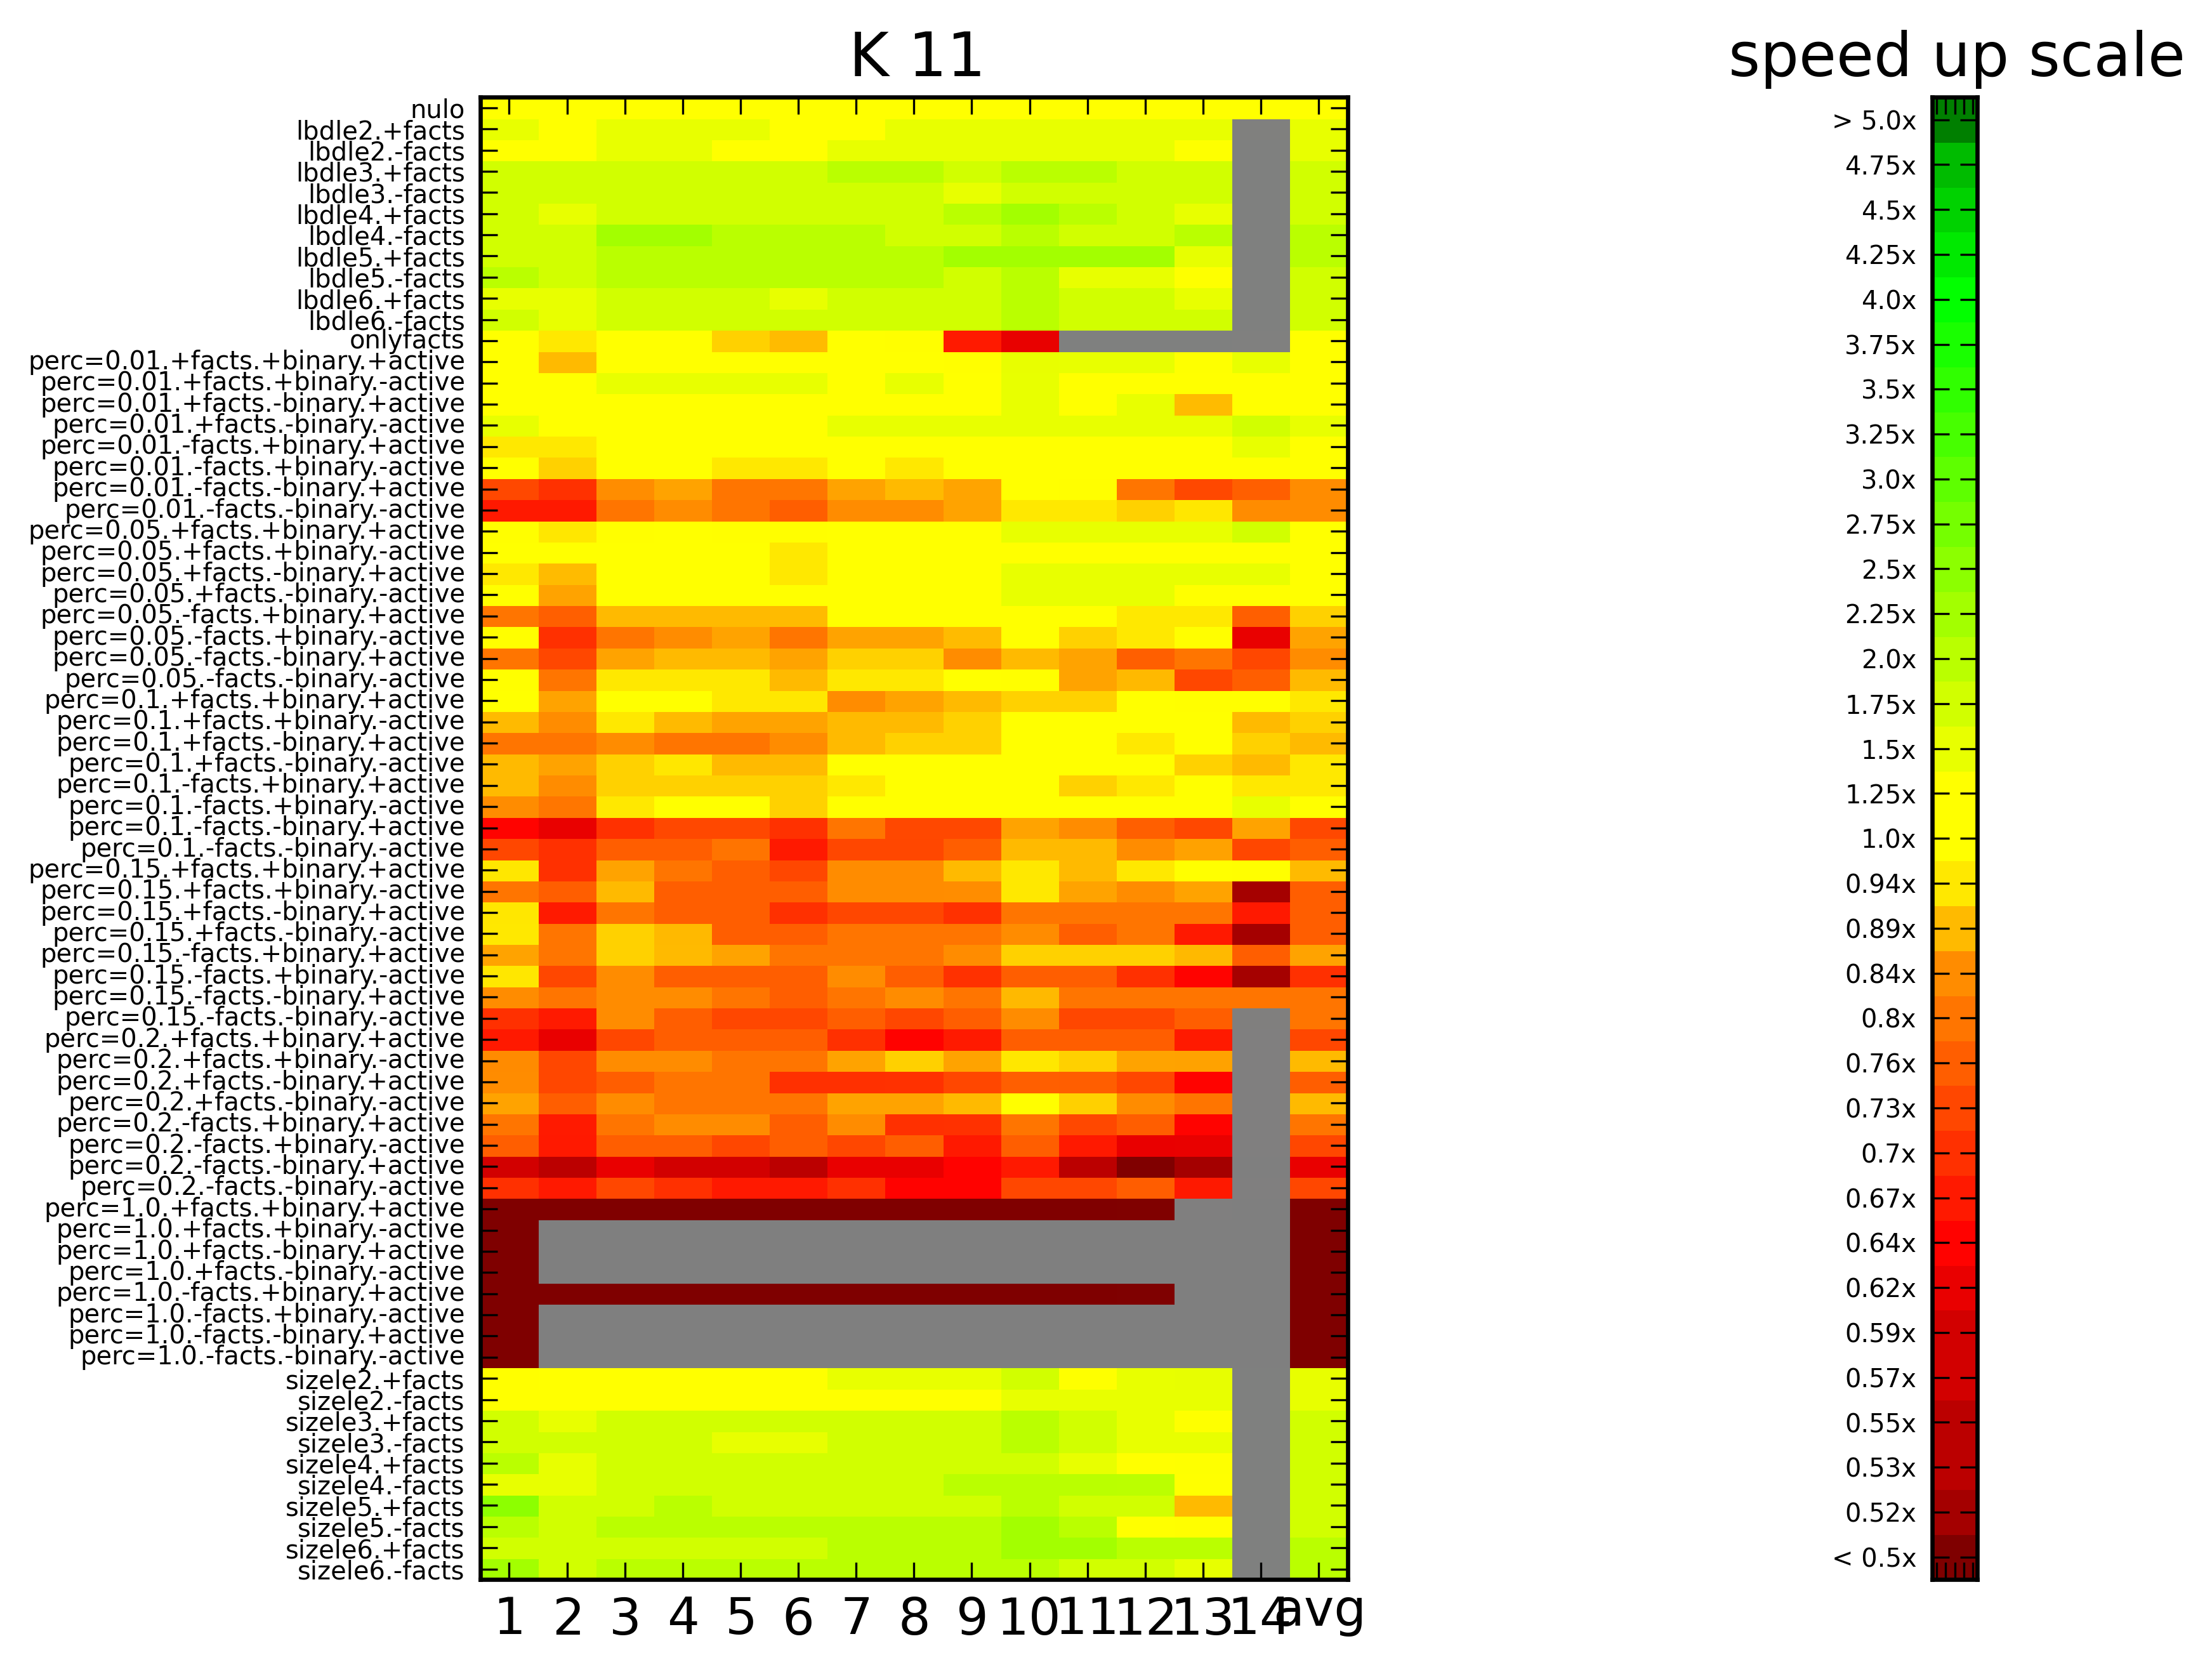
\includegraphics[scale=0.5]{resultados/k11_heat}
% 	%\caption{\emph{Workers}}
% \end{figure}
% \begin{figure}
% 	\centering
% 	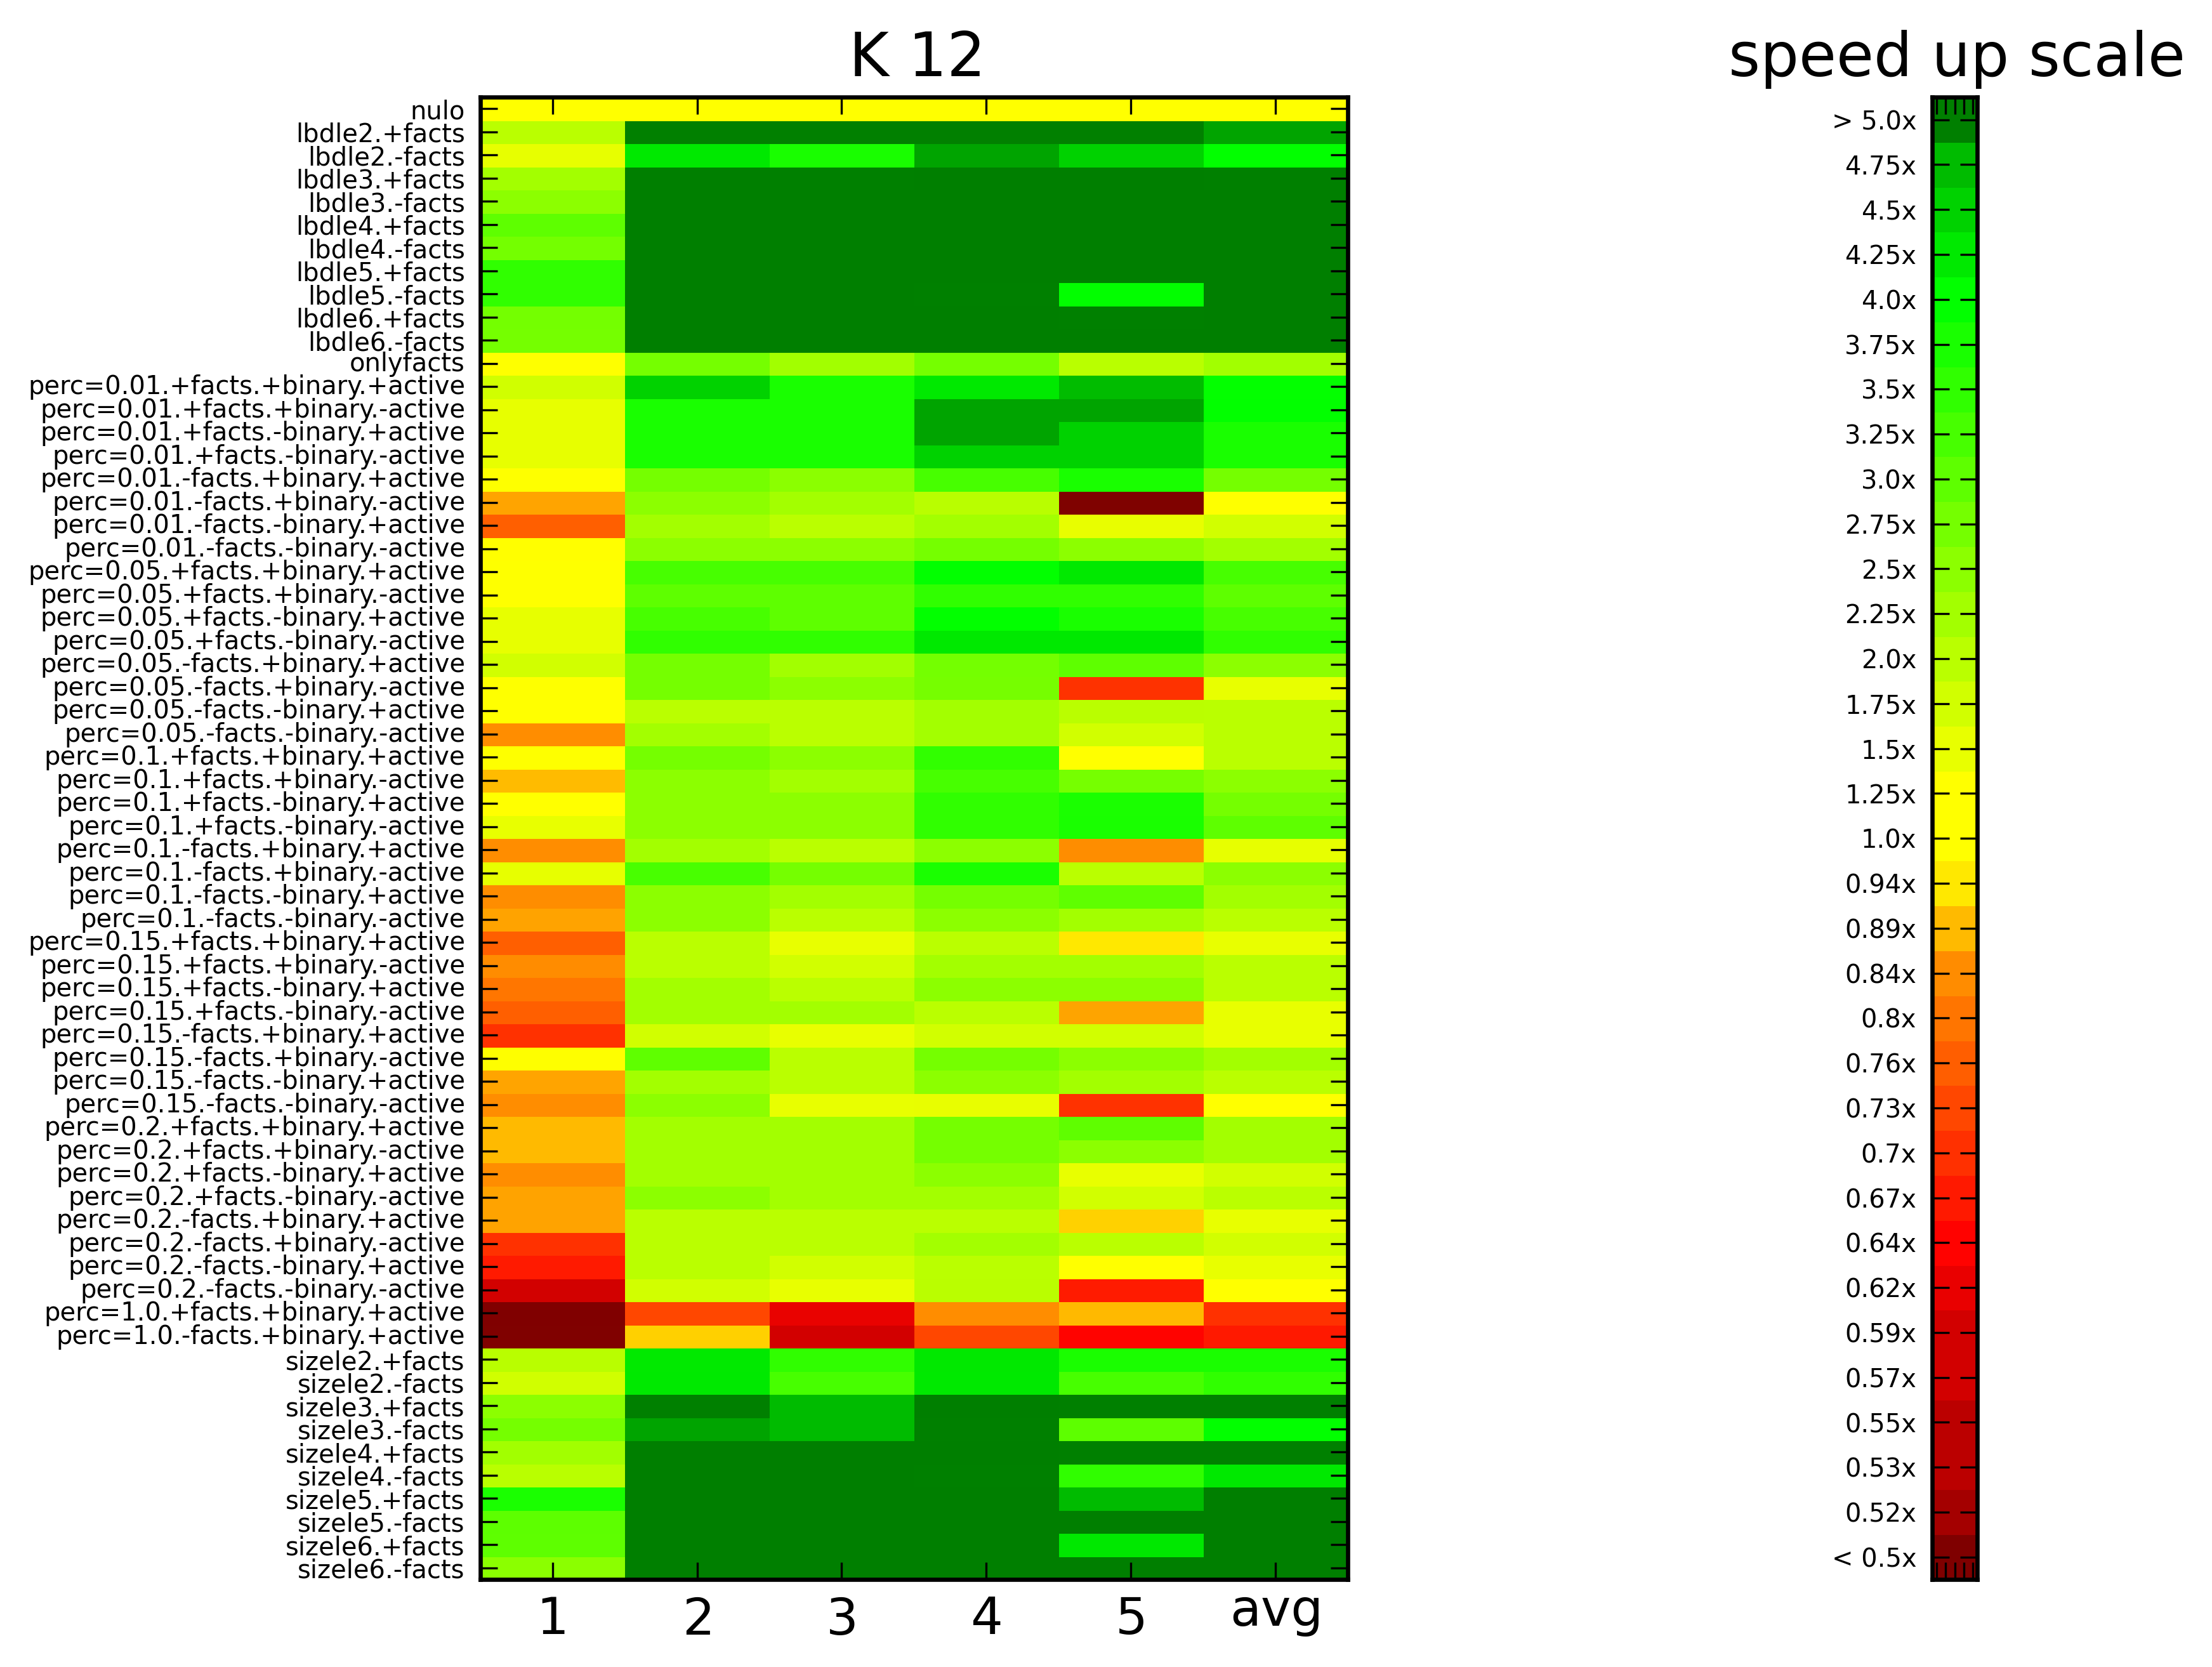
\includegraphics[scale=0.6]{resultados/k12_heat}
% 	%\caption{\emph{Workers}}
% \end{figure}
% \begin{figure}
% 	\centering
% 	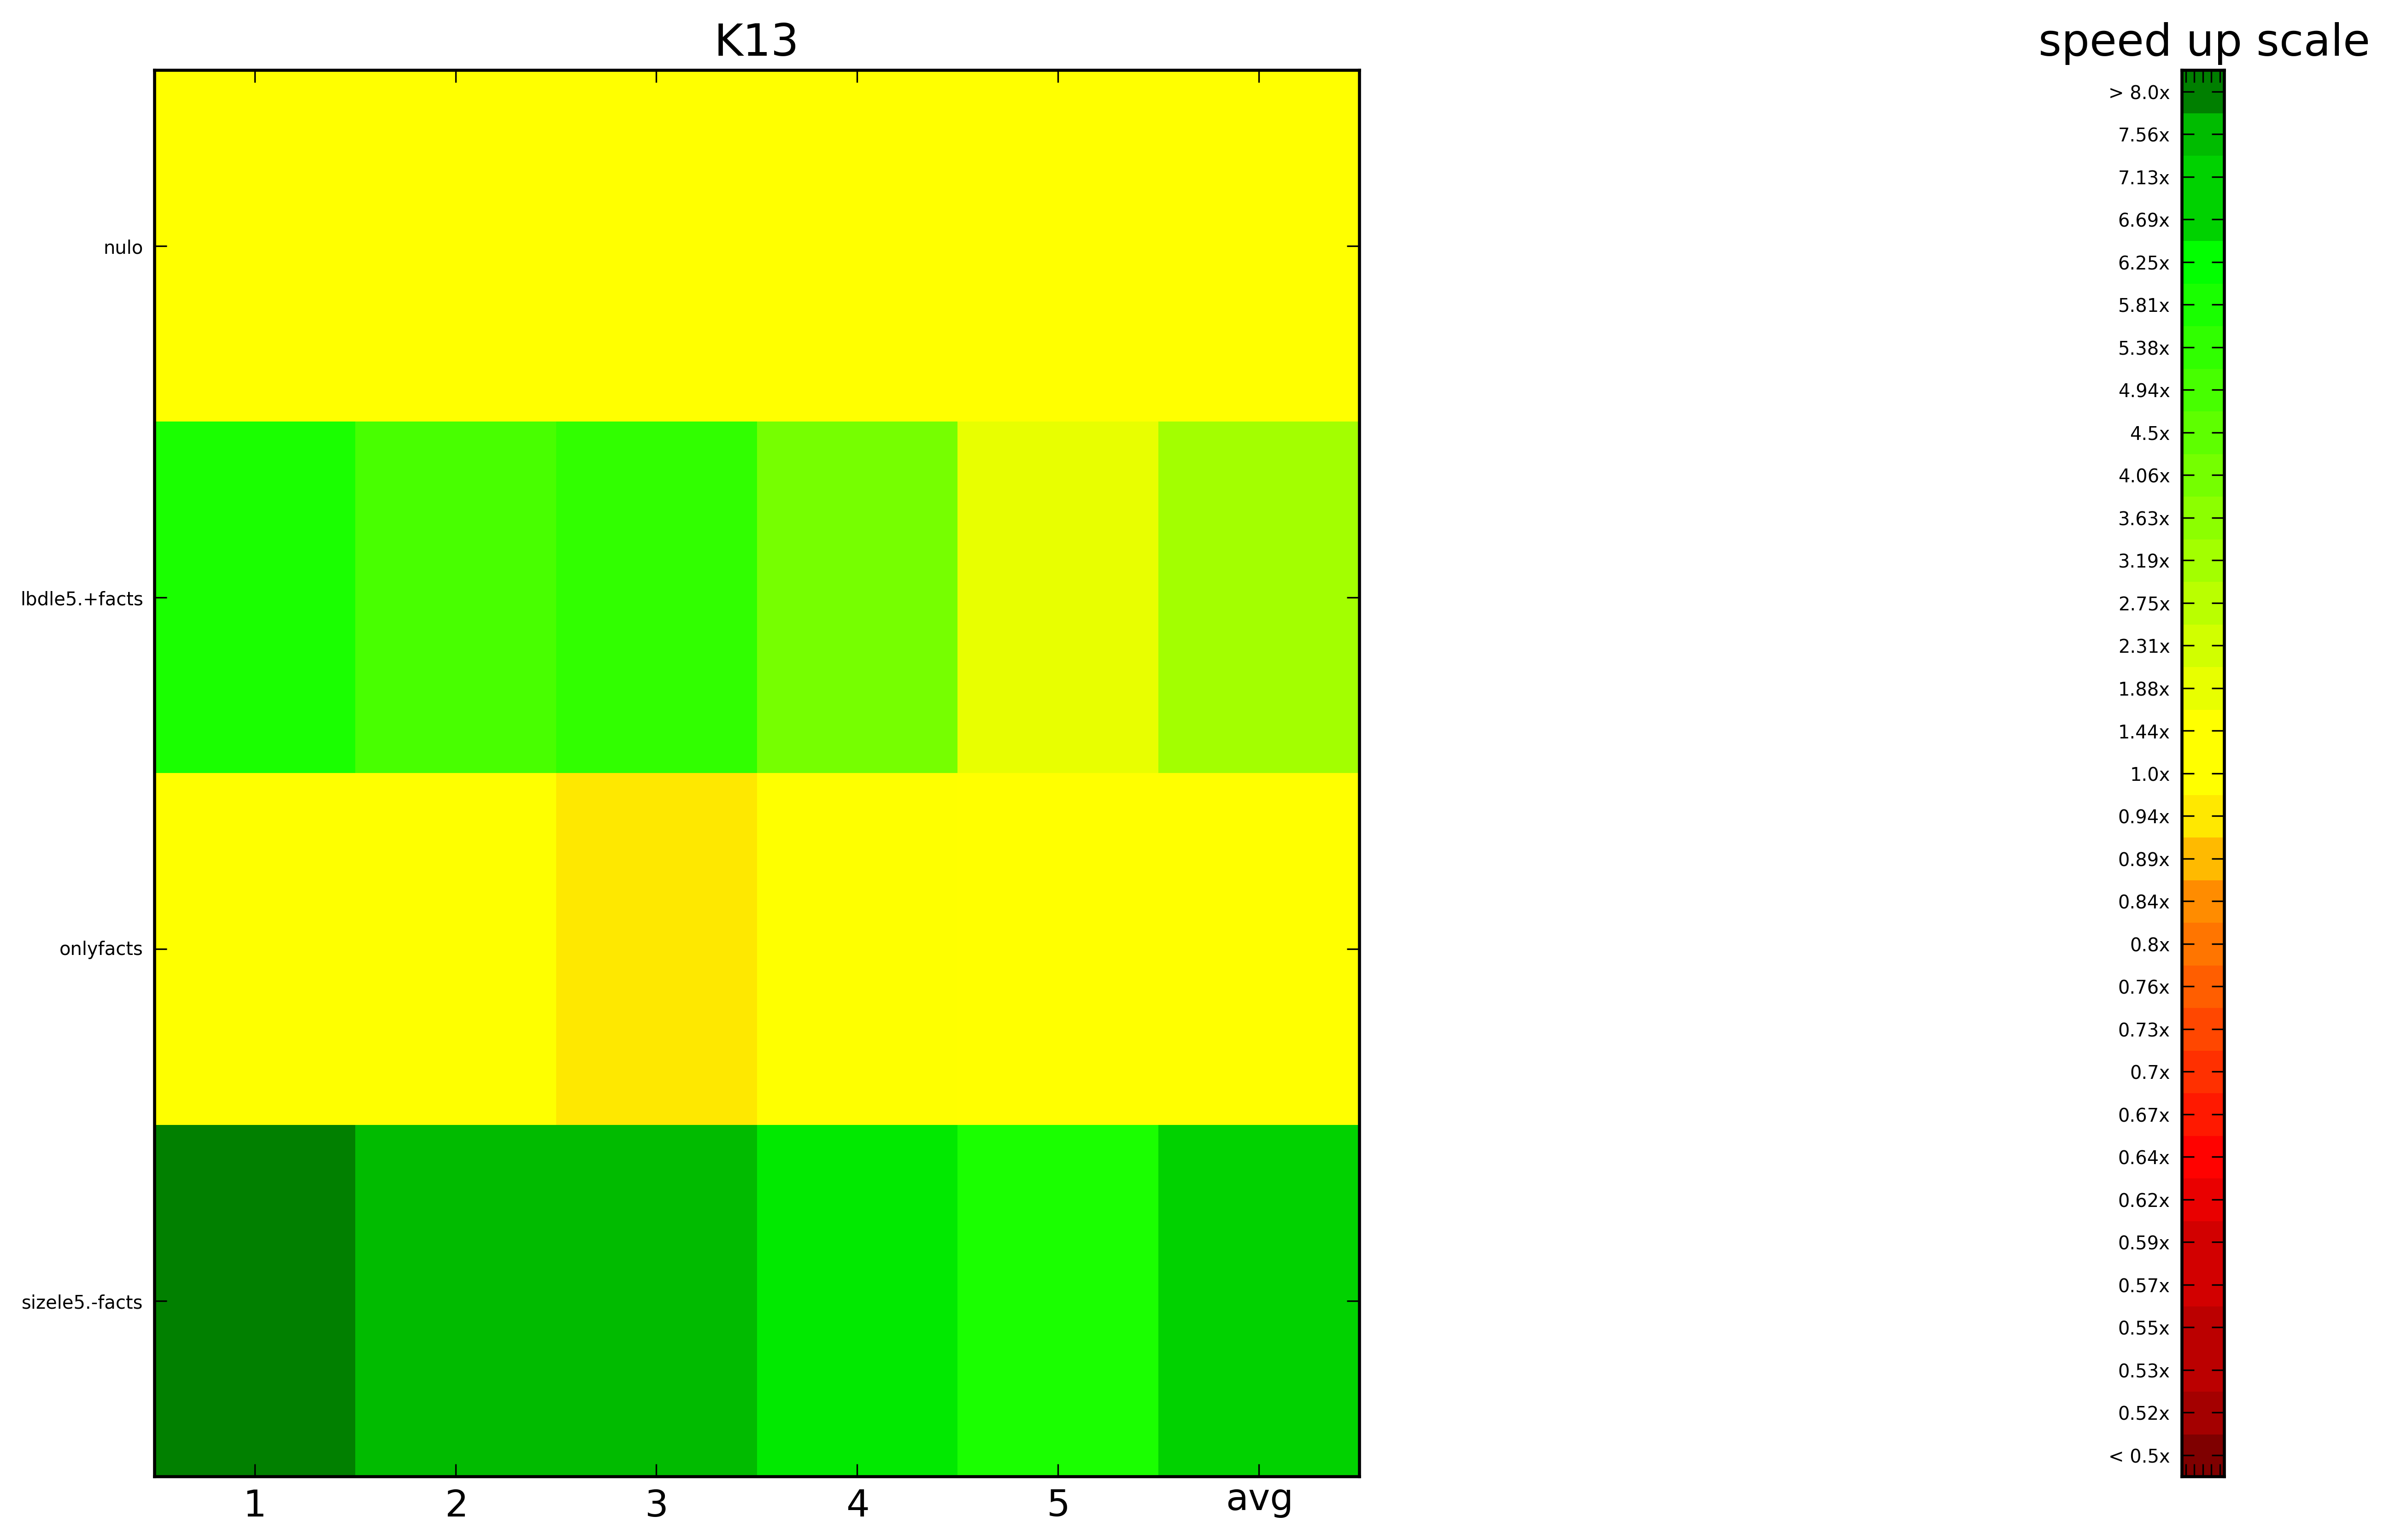
\includegraphics[scale=0.6]{resultados/k13_heat}
% 	%\caption{\emph{Workers}}
% \end{figure}

\hspace{-5em}
\begin{minipage}{\textwidth}
	\small
	\begin{tabular}{lrrr}
		\toprule
		criteria	&	worst speedup (x)	&	best speedup (x)	&	avg speedup (x) \\
		\cmidrule(r){1-4}
		lbdle2.+facts	&	0.68	&	4.91	&	1.97 \\
		lbdle2.-facts	&	0.71	&	3.84	&	1.24 \\
		lbdle3.+facts	&	0.78	&	5.16	&	1.41 \\
		lbdle3.-facts	&	0.75	&	5.71	&	1.69 \\
		lbdle4.+facts	&	0.64	&	6.80	&	1.68 \\
		lbdle4.-facts	&	0.79	&	5.83	&	1.83 \\
		lbdle5.+facts	&	0.69	&	6.74	&	1.64 \\
		lbdle5.-facts	&	0.77	&	5.25	&	2.14 \\
		lbdle6.+facts	&	0.76	&	5.79	&	1.95 \\
		lbdle6.-facts	&	0.70	&	6.08	&	1.94 \\
		\cmidrule(r){1-4}
		onlyfacts	&	\cellcolor{green}0.84	&	3.23	&	1.45 \\
		\cmidrule(r){1-4}
		perc=0.01.+facts.+binary.+active	&	\cellcolor{red}0.55	&	3.83	&	2.12 \\
		perc=0.01.+facts.+binary.-active	&	0.77	&	3.78	&	1.92 \\
		perc=0.01.+facts.-binary.+active	&	0.64	&	3.64	&	\cellcolor{red}1.19 \\
		perc=0.01.+facts.-binary.-active	&	0.65	&	3.50	&	1.39 \\
		perc=0.01.-facts.+binary.+active	&	0.74	&	2.73	&	1.91 \\
		perc=0.01.-facts.+binary.-active	&	0.69	&	2.38	&	1.30 \\
		perc=0.01.-facts.-binary.+active	&	0.74	&	\cellcolor{red}1.68	&	1.22 \\
		perc=0.01.-facts.-binary.-active	&	0.71	&	2.22	&	1.22 \\
		\cmidrule(r){1-4}
		sizele2.+facts	&	0.75	&	3.50	&	1.57 \\
		sizele2.-facts	&	0.81	&	3.32	&	\cellcolor{red}1.19 \\
		sizele3.+facts	&	\cellcolor{red}0.55	&	5.40	&	1.63 \\
		sizele3.-facts	&	0.75	&	3.87	&	1.39 \\
		sizele4.+facts	&	0.74	&	6.24	&	1.91 \\
		sizele4.-facts	&	0.72	&	4.21	&	1.81 \\
		sizele5.+facts	&	0.64	&	6.14	&	1.92 \\
		sizele5.-facts	&	0.58	&	\cellcolor{green}7.18	&	1.90 \\
		sizele6.+facts	&	0.72	&	5.08	&	2.17 \\
		sizele6.-facts	&	0.79	&	5.69	&	\cellcolor{green}2.61 \\
		\bottomrule
	\end{tabular}
	%\caption{Tiempo de ejecución (en segundos) distribuido vs. secuencial}
\end{minipage}



